\documentclass[12pt]{article}
\usepackage[utf8]{inputenc}
\usepackage{lipsum}
\usepackage{pifont}
\usepackage{outlines}
\usepackage{multirow}
\usepackage{multicol}
\usepackage{subcaption}
\usepackage{adjustbox}
\usepackage{amsmath}
\usepackage{makecell}
\usepackage{fancyhdr}
\usepackage{float}
\usepackage{graphicx}
\usepackage{tikz,xcolor}
\usepackage{karnaugh-map}
\usepackage{longtable}
\usepackage{hyperref}
\setlength{\columnseprule}{0.4pt}
\usepackage[a4paper, total={7in, 10in}]
{geometry}

\usepackage[skip =10pt, indent =0pt]{parskip}

\pagestyle{fancy}
\fancyhead[C]{Computer Architecture Sessional Assignment 1}
\fancyhead[R]{}
\fancyhead[L]{CSE 306}
\fancyfoot[R]{Prepared using \LaTeX}

\title{CSE 306 OFFLINE 3 LABORATORY REPORT}
\author{\textsuperscript{1}Sadia Tabassum, \textsuperscript{2}Alina Zaman, \textsuperscript{3}Md.Shafiul Haque ,\\\textsuperscript{4}Mayesha Rashid, \textsuperscript{5}Saha Kuljit Shantanu}
\date{1 March 2022}





\begin{document}

\maketitle

\section{Introduction}

A \textit{4 bit MIPS} is a instruction set that contains a databus of only 4 bits, that is , a register can store only four bits of data(Signed or Unsigned) in it.

For this assignment, we have done or attempted the following things:
\begin{itemize}
    \item Designing a 4 bit MIPS structure with assigned 16-bit instruction set
    \item Simulating the design in a simulating software(In our case we hve used Logisim-win-2.7.1)
    \item Implementing the design in hardwares
\end{itemize}

\section{Properties of our Instruction Set Architecture}

For this assignment, our instruction set is of following features:
\begin{itemize}
    \item It is a 16-bit instruction set
    \item Operational code is of 4 bit
    \item The data bus are 4 bits each and the address bus is 8 bits
    \item The conditional Jumps are of 4 bit offset
    \item Only logical shift is implemented
    \item The shift amount for logical shifts is of 4 bit 
    \item The register identifiers are of 4 bit
    \item The following registers are used: 
\begin{multicols}{4}
    \subitem \textbf{\$zero}
    \subitem \textbf{\$t0}
    \subitem \textbf{\$t1}
    \subitem \textbf{\$t2}
    \subitem \textbf{\$t3}
    \subitem \textbf{\$t4}
    \subitem \textbf{\$sp}
    \subitem \textbf{\$ra}
    \subitem \textbf{\$a0}
    \subitem \textbf{\$a1}
    \subitem \textbf{\$v0}
    \subitem \textbf{\$v1}
    \subitem \textbf{\$s0}
    \subitem \textbf{\$s1}

\end{multicols}

\item The following instructions are implemented(In Opcode Order) :
\begin{multicols}{2}

    \subitem \textbf{sub}
    \subitem \textbf{lw}
    \subitem \textbf{bneq}
    \subitem \textbf{beq}
    \subitem \textbf{j, jal(Shared opcode)}
    \subitem \textbf{ori}
    \subitem \textbf{add}
    \subitem \textbf{subi}
    \subitem \textbf{andi}
    \subitem \textbf{sw}
    \subitem \textbf{nor}
    \subitem \textbf{addi}
    \subitem \textbf{or}
    \subitem \textbf{srl}
    \subitem \textbf{sll}
    \subitem \textbf{and,jr(Shared opcode)}
    
\end{multicols}
    
\end{itemize}

\begin{table}[H]
    \centering
    \begin{tabular}{|l|c|c|c|c|}

        \hline
        \textbf{Instruction Type} & \textbf{BIT15 to BIT12} & \textbf{BIT11 to BIT8} & \textbf{BIT7 to BIT4} & \textbf{BIT3 to BIT0} \\
        \hline
        \textbf{R-type} & \multirow{6}{*}{Opcode} & \multirow{5}{*}{SrcReg1} & SrcReg2 & DstReg\\
        \cline{1-1}
        \cline{4-5}
        \textbf{S-type} &  &  & DstReg & ShAmt\\
        \cline{1-1}
        \cline{4-5}
        \textbf{I-type(memory)} &  &  & MemReg & \multirow{2}{*}{Offset}\\
        \cline{1-1}
        \cline{4-4}
        \textbf{I-type(branch)} &  &  & SrcReg2 & \\
        \cline{1-1}
        \cline{4-5}
        \textbf{I-type(AL)} &  &  & DstReg & Immediate\\
        \cline{1-1}
        \cline{3-5}
        \textbf{J-type} &  & \multicolumn{2}{|c|}{Target Jump Address} & Reusable\\
        \hline
    \end{tabular}
    \caption{Instruction Set Structure for various types}
    \label{tab:t1}
\end{table}

\section{Instruction Sets}

\subsection{Opcode Specific Instructions(Opcode Ordered)}

%CLONPHADFMKBGJIE

\begin{table}[H]
    \centering
    \begin{tabular}{|c|c|c|c|c|}

        \hline
        \textbf{Instruction} & \textbf{Opcode} & \textbf{Istruction type} & \textbf{Instruction ID} & \textbf{Task type} \\
        \hline
        \textbf{sub} & 0000 & Arithmetic & C & R-type\\
        \hline
        \textbf{lw} & 0001 & Memory & L & I-type\\
        \hline
        \textbf{bneq} & 0010 & Control & O & I-type\\
        \hline
        \textbf{beq} & 0011 & Control & N & I-type\\
        \hline
        
        \textbf{j} & 0100 & Control & P & J-type\\
        \hline
        \textbf{ori} & 0101 & Logic & H & I-type\\
        \hline
        \textbf{add} & 0110 & Arithmetic & A & R-type\\
        \hline
        \textbf{subi} & 0111 & Arithmetic & D & I-type\\
        \hline
        
        \textbf{andi} & 1000 & Logic & F & I-type\\
        \hline
        \textbf{sw} & 1001 & Memory & M & I-type\\
        \hline
        \textbf{nor} & 1010 & Logic & K & R-type\\
        \hline
        \textbf{addi} & 1011 & Arithmetic & B & I-type\\
        \hline
        
        \textbf{or} & 1100 & Logic & G & R-type\\
        \hline
        \textbf{srl} & 1101 & Logic & J & S-type\\
        \hline
        \textbf{sll} & 1110 & Logic & I & S-type\\
        \hline
        \textbf{and} & 1111 & Logic & E & R-type\\
        \hline
    \end{tabular}
    \caption{Opcode specific Instruction Set}
    \label{tab:t2}
\end{table}

\subsection{Set Specific Instructions(Opcode Shared)}

\begin{table}[H]
    \centering
    \begin{tabular}{|c|c|c|c|c|}
        \hline
        \textbf{Instruction Name} & \textbf{BIT15 to BIT12} & \textbf{BIT11 to BIT8} & \textbf{BIT7 to BIT4} & \textbf{BIT3 to BIT0} \\
        \hline
        \textbf{jal} & 4 & \multicolumn{2}{|c|}{Jump Address} & Self Address\\
        \hline    
        \textbf{jr} & F &  F & F & 7(recognizer for \textbf{\$ra})\\
        \hline
    \end{tabular}
    \caption{Set Specific Instruction Set}
    \label{tab:t3}
\end{table}

\section{Register Set}

\begin{table}[H]
    \centering
    \begin{tabular}{|c|c|c|}
    \hline
    \textbf{Register} & \textbf{Recognizer} & \textbf{Register Type}\\
    \hline
    \textbf{\$zero} & 0000 & Zero \\
    \hline
    \textbf{\$t0} & 0001 & \multirow{5}{*}{Temporary} \\
    \cline{1-2}
    \textbf{\$t1} & 0010 &  \\
    \cline{1-2}
    \textbf{\$t2} & 0011 &  \\
    \cline{1-2}
    \textbf{\$t3} & 0100 &  \\
    \cline{1-2}
    \textbf{\$t4} & 0101 &  \\
    \hline
    \textbf{\$sp} & 0110 & Stack Pointer \\
    \hline
    \textbf{\$ra} & 0111 & Return Address\\
    \hline
    \textbf{\$a0} & 1000 & \multirow{2}{*}{Argument} \\
    \cline{1-2}
    \textbf{\$a1} & 1001 &  \\
    \hline
    \textbf{\$v0} & 1010 & \multirow{2}{*}{Return} \\
    \cline{1-2}
    \textbf{\$v1} & 1011 &  \\
    \hline
    \textbf{\$s0} & 1100 & \multirow{2}{*}{Saved} \\
    \cline{1-2}
    \textbf{\$s1} & 1101 &  \\
    \hline
    \end{tabular}
    \caption{Register Set}
    \label{tab:t4}
\end{table}

\section{Components in implementation of Project}

\begin{itemize}
    \item [\ding{227}] An assembler code written in c++ to convert user provided assembly code to machine language ( \textit{MIPS instruction Set} )
    \item [\ding{227}] A simulator (\textit{logisim-win-2.7.1})
    \item[\ding{227}] 5 Atmega for hardware implementation and their codes
    \item[\ding{227}] D- flipflops, Push switches, Logic and Arithmetic IC's, Jumper wires and Professional wires\\
\end{itemize}

\section{Block and DataPath Analysis}

    \begin{figure}[H]
        \centering
        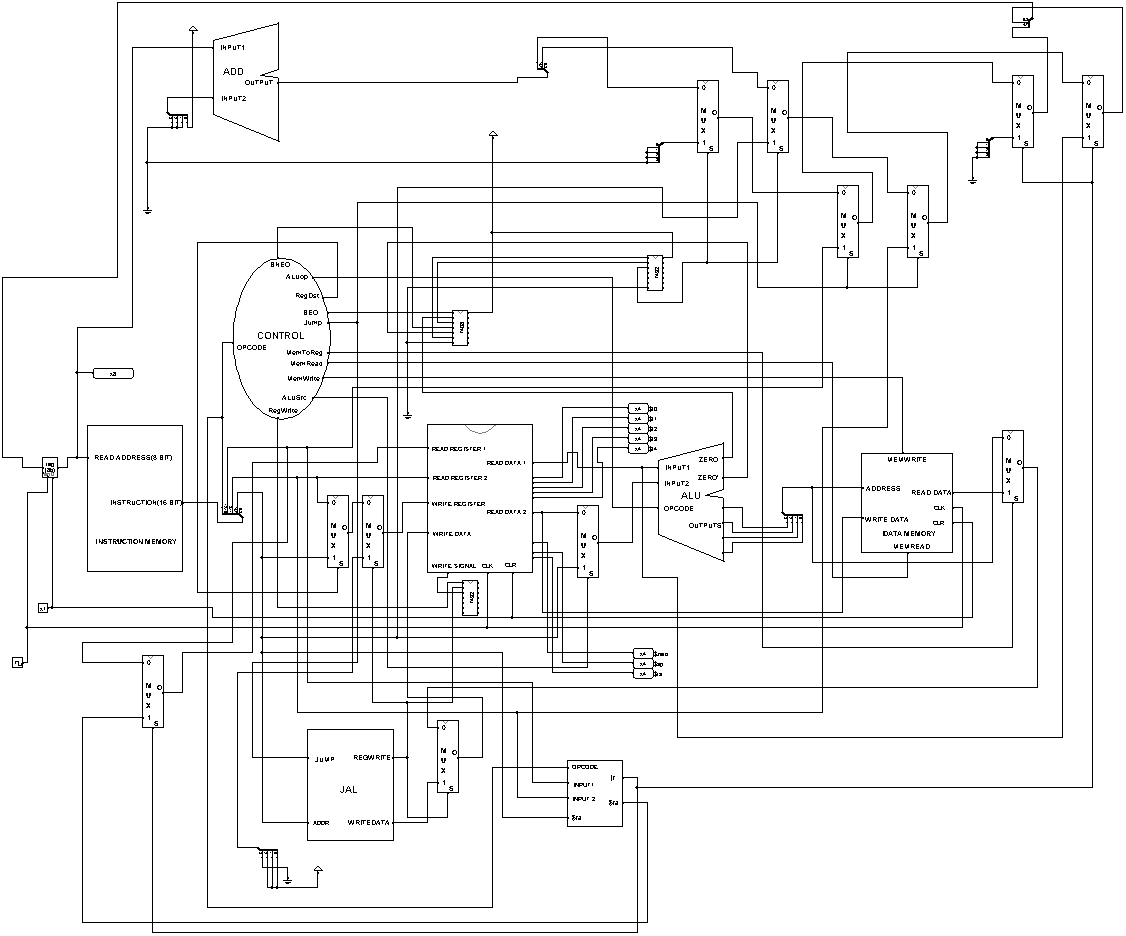
\includegraphics[width = 0.9\textwidth]{DATAPATH.png}
        \caption{\textbf{Overall DataPath}}
        \label{fig:1}
    \end{figure}

   
\subsection{Instruction Memory}

    In the instruction memory, we have an \textit{EEPROM} that takes a \textbf{8 bit address} as input and \textbf{16 bit data} as output. Here the 
    \textbf{8 bit address} is the \textbf{Program Counter}, while each \textbf{16 bit data } denotes an {instruction set}.

     \begin{figure}[H]
        \centering
        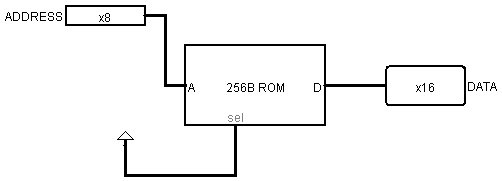
\includegraphics{INSTRUCTION MEMORY.png}
        \caption{\textbf{Instruction Memory}}
        \label{fig:2}
    \end{figure}

\subsection{Control Unit}  


\subsubsection{Opcode Dependent Control}
In the Control Unit, we have a \textit{decoder} that takes the \textbf{4 bit Opcode} as input and \textbf{1 bit control} as output. Here the \textbf{4 bit Opcode} passes to the \textbf{ALU}.The opcode is decoded and then by \textbf{OR} logic, the Controls are generated. The functions of the Controls will be discussed in section \textbf{9}.
\begin{table}[H]
    \centering
    \begin{adjustbox}{width=\textwidth}
        \begin{tabular}{|c|c|c|c|c|c|c|c|c|c|c|}
            \hline
            \textbf{Instruction} & \textbf{Opcode} &  \textbf{RegDst} & \textbf{BranchEqual} & \textbf{BranchnotEqual} & \textbf{Jump} & \textbf{MemtoReg} & \textbf{MemRead} & \textbf{MemWrite} & \textbf{ALUSrc} & \textbf{RegWrite}\\
            \hline 
            \textbf{sub} & 0000 & 1 & 0 & 0 & 0 & 0 & 0 & 0 & 0 & 1 \\
            \hline
            \textbf{}lw & 0001 & 0 & 0 & 0 & 0 & 1 & 1 & 0 & 1 & 1 \\
            \hline
            \textbf{bneq} & 0010 & 1 & 0 & 1 & 0 & 0 & 0 & 0 & X & 0 \\
            \hline
            \textbf{beq} & 0011 & 1 & 1 & 0 & 0 & 0 & 0 & 0 & X & 0 \\
            \hline
            \textbf{j} & 0100 & X & X & X & 1 & 0 & 0 & 0 & X & 0 \\
            \hline
            \textbf{ori} & 0101 & 0 & 0 & 0 & 0 & 0 & 0 & 0 & 1 & 1 \\
            \hline
            \textbf{add} & 0110 & 1 & 0 & 0 & 0 & 0 & 0 & 0 & 0 & 1 \\
            \hline
            \textbf{subi} & 0111 & 0 & 0 & 0 & 0 & 0 & 0 & 0 & 1 & 1 \\
            \hline
            \textbf{andi} & 1000 & 0 & 0 & 0 & 0 & 0 & 0 & 0 & 1 & 1 \\
            \hline
            \textbf{sw} & 1001 & 0 & 0 & 0 & 0 & 0 & 0 & 1 & 1 & 0 \\
            \hline
            \textbf{nor} & 1010 & 1 & 0 & 0 & 0 & 0 & 0 & 0 & 0 & 1 \\
            \hline
            \textbf{addi} & 1011 & 0 & 0 & 0 & 0 & 0 & 0 & 0 & 1 & 1 \\
            \hline
            \textbf{or} & 1100 & 1 & 0 & 0 & 0 & 0 & 0 & 0 & 0 & 1 \\
            \hline
            \textbf{srl} & 1101 & 0 & 0 & 0 & 0 & 0 & 0 & 0 & 1 & 1 \\
            \hline
            \textbf{sll} & 1110 & 0 & 0 & 0 & 0 & 0 & 0 & 0 & 1 & 1 \\
            \hline
            \textbf{and} & 1111 & 1 & 0 & 0 & 0 & 0 & 0 & 0 & 0 & 1 \\
            \hline
            
        \end{tabular}
    \end{adjustbox}
    \caption{Control(Opcode Ordered)}
    \label{tab:t5}
\end{table}

    \begin{figure}[H]
        \centering
        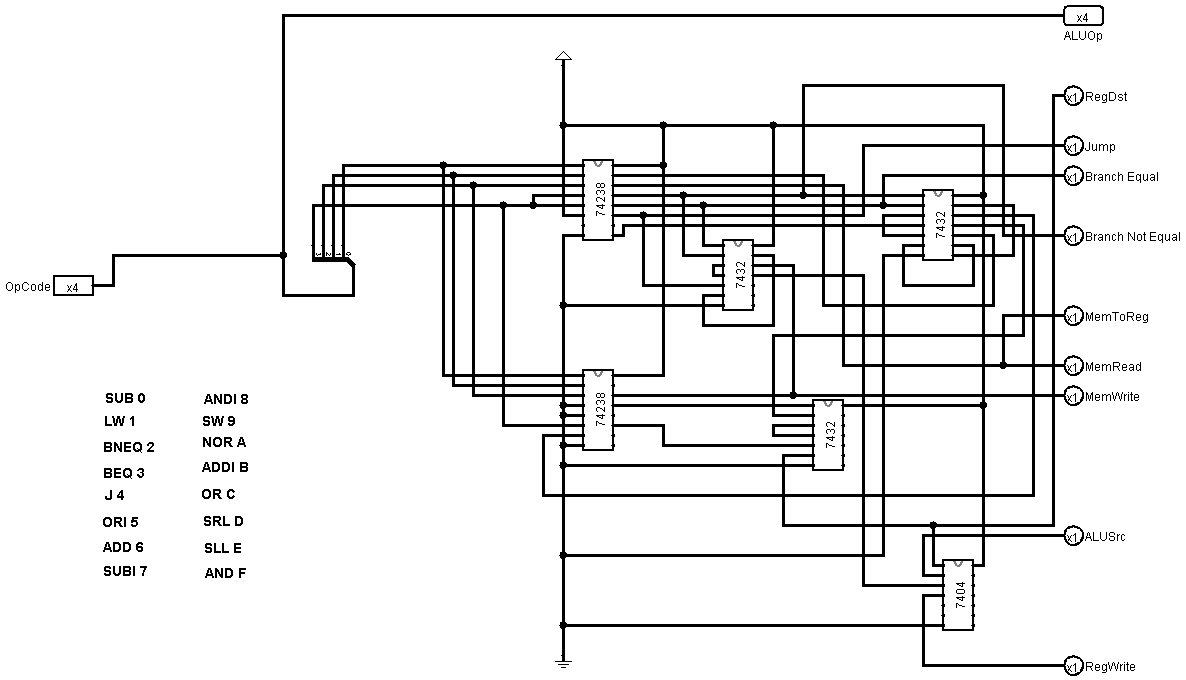
\includegraphics[width = 0.9\textwidth]{CONTROL.png}
        \caption{\textbf{Control}}
        \label{fig:3}
    \end{figure}

\subsubsection{Additional Controls}

\tikzstyle{arrow} = [thick,->,>=stealth]
\tikzstyle{block} = [rectangle, 
minimum height= 5cm,
minimum width= 5cm, 
text centered, 
draw=black, 
fill=white!30]

\tikzstyle{sblock} = [rectangle, 
minimum height= 3cm,
minimum width= 3cm, 
text centered, 
draw=black, 
fill=white!30]

\tikzstyle{lblock} = [rectangle, 
minimum height= 13cm,
minimum width= 10cm, 
text centered, 
draw=red!200, 
%dotted,
fill=white!30]

\tikzstyle{io} = [rectangle, 
minimum height= 1cm,
minimum width= 1cm, 
text centered, 
draw=black, 
fill=white!30]

\begin{itemize}
    \item \textbf{JAL\_Control : } This control is dependent on the Jump control and the value of \textbf{\$ra} register. 

    \begin{table}[H]
        \centering
        \begin{tabular}{|c|c|c|c|}
             \hline
             \textbf{Jump} & \textbf{BIT3-BIT0 of Instruction set} & 
             \textbf{RegWrite} & \textbf{Data to be put in \$ra}  \\
             \hline
             0 & (X)\textsubscript{H} & 0 & 0 \\
             \hline
             1 & (0)\textsubscript{H} & 0 & 0 \\
             \hline
             1 & Y\textsubscript{H}(can be anything but 0) & 1 & Y\textsubscript{H} \\
             \hline
        \end{tabular}
        \caption{JAL Control Truth Table}
        \label{tab:t6}
    \end{table}

    \begin{tikzpicture}

        \node (in1) [io]{JUMP};
        \node (in2) [io,below of = in1,yshift = -3cm]{BIT3-BIT0};
        \node (jal) [block, right of =in1, xshift = 5cm, yshift = -2cm] {JAL Control};

        \draw [arrow] (in1) -- ++(3.5,0);
        \draw [arrow] (in2) -- ++(3.5,0);

        \node (out1) [io,right of =in1, xshift = 11cm]{RegWrite};
        \node (out2) [io,below of = out1,yshift = -3cm]{Self Address for \$ra};
        
        \draw [arrow] (in1)++(8.5,0) -- (out1);
        \draw [arrow] (in2)++(8.5,0) -- (out2);
    \end{tikzpicture}

    

    \begin{tikzpicture}

        %\textbf{Writing Register \$ra by jal:}

        \node (in1) [io]{RegWrite from JAL Control};
        \node (in2) [io,below of = in1,yshift = -3cm]{RegWrite from Control};
        \node (or) [block, right of =in1, xshift = 5cm, yshift = -2cm] {OR gate};

        \draw [arrow] (in1) -- ++(3.5,0);
        \draw [arrow] (in2) -- ++(3.5,0);

        \node (out1) [block,right of =or, xshift = 5cm]{\textbf{Register}};
        \draw [arrow] (or) -- (out1);

        \node (in3) [io,below of = out1, yshift = -5cm]{Self Address for \$ra};
        \draw [arrow] (in3) -- (out1);
        \node (in4) [io,above of = out1, yshift = 5cm]{0111};
        \draw [arrow] (in4) -- (out1);
        \node [below of = out1,yshift = -1cm]{WriteData};
        \node [above of = out1,yshift = 1cm]{WriteRegister};
        \node [left of = out1,xshift = -0.9cm]{Signal};
        \node [below of = or,yshift = -7cm]{\textbf{Writing Register \$ra by jal}}
        
        %\caption{RegWrite by jal}

    \end{tikzpicture}

    \begin{figure}[H]
        \centering
        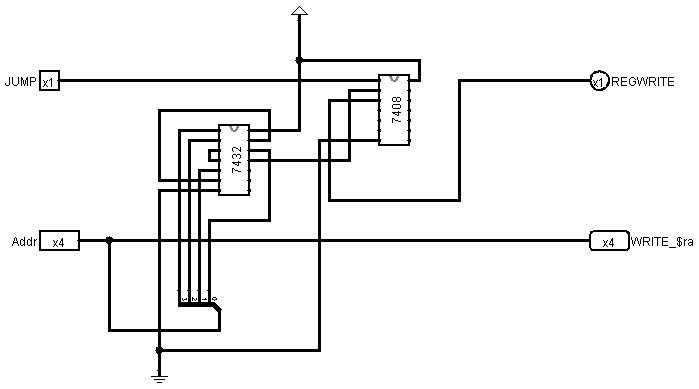
\includegraphics[width = 0.9\textwidth]{JAL_CONTROL.png}
        \caption{\textbf{Jump And Link Control}}
        \label{fig:4}
    \end{figure}
    
    \item \textbf{JR\_Control : } This control will take 16 bit data as input and give JR flag as output.\\
    Apparently, it will be activated only when it gets FFF7 as input. Only when it gets FFF, JR becomes 1. JR activates Jump by doing OR to the jump flag.
    And it takes the value in register7(\textbf{\$ra}) to jump at that address \\ \\ \\

    \begin{figure}[H]
        \centering
        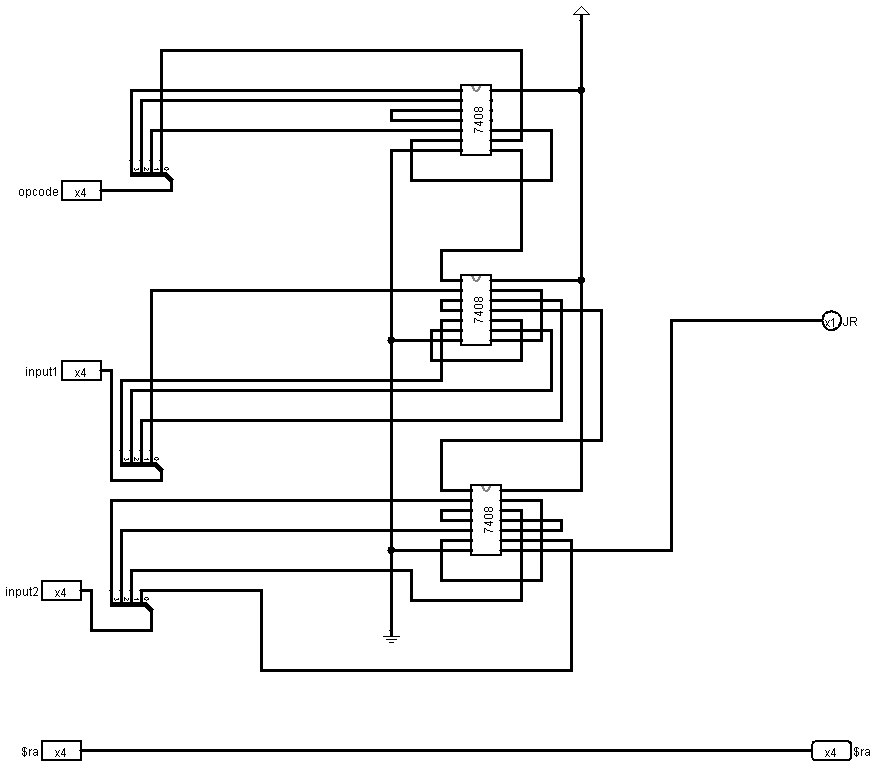
\includegraphics[width = 0.9\textwidth]{JR.png}
        \caption{\textbf{Jump Return Control}}
        \label{fig:5}
    \end{figure}

    
\end{itemize}
\subsection{Register File}

    

    \begin{figure}[H]
        \centering
        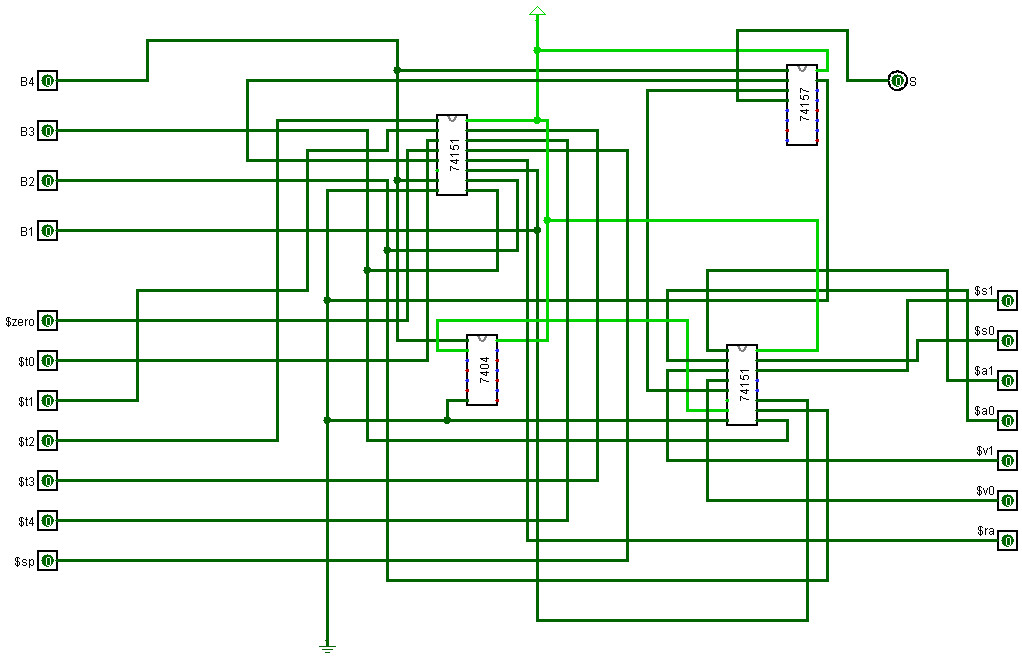
\includegraphics[width = 0.9\textwidth]{READ_SELECTER.png}
        \caption{\textbf{Read Selector}}
        \label{fig:6}
    \end{figure}

    In register file, 2 registers of 4bit can be read at a time, while only one register can be written. 
    \begin{itemize}
            \item Whether to write in a register is controled by a write signal. If an instruction intends to write some data into the register, then the \textbf{regWrite} for that control signal will be 1.
            \item To determine whether the BIT7-BIT4 will be the register to write(S or I type) or the BIT3-BIT0 are the destination registers(R type), this decision is made by \textbf{RegDst} .
    \end{itemize}

     \begin{figure}[H]
        \centering
        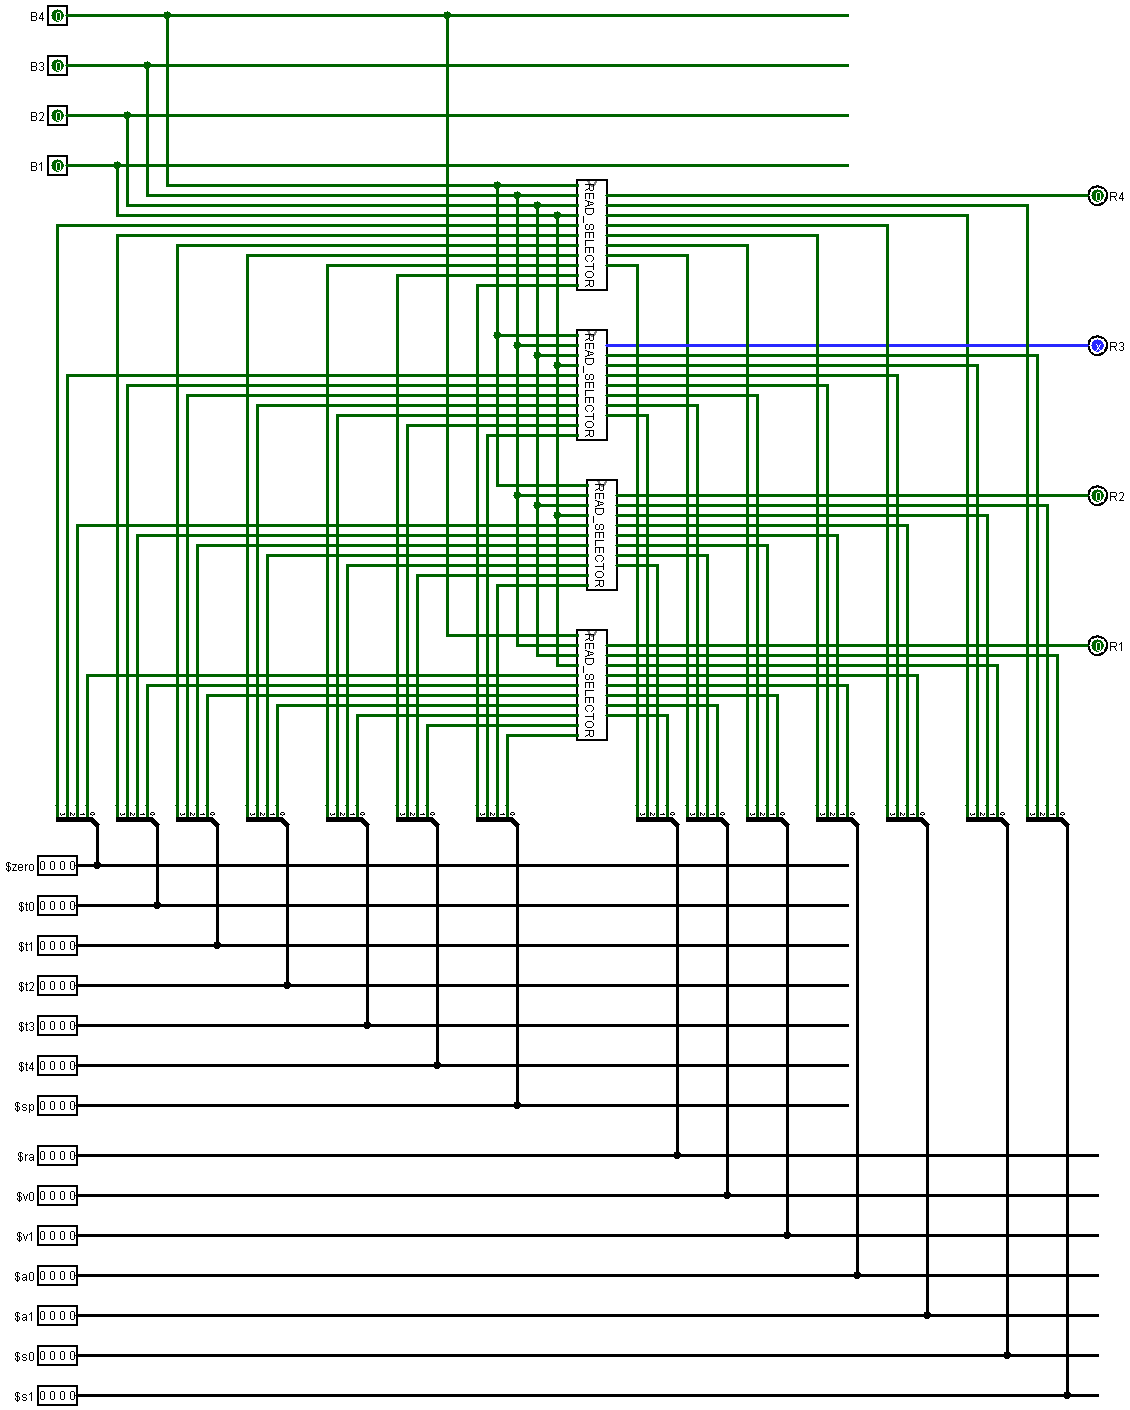
\includegraphics[width = 0.9\textwidth ]{READ_REGISTER_CIRCUIT.png}
        \caption{\textbf{Reader}}
        \label{fig:7}
    \end{figure}

    \begin{figure}[H]
        \centering
        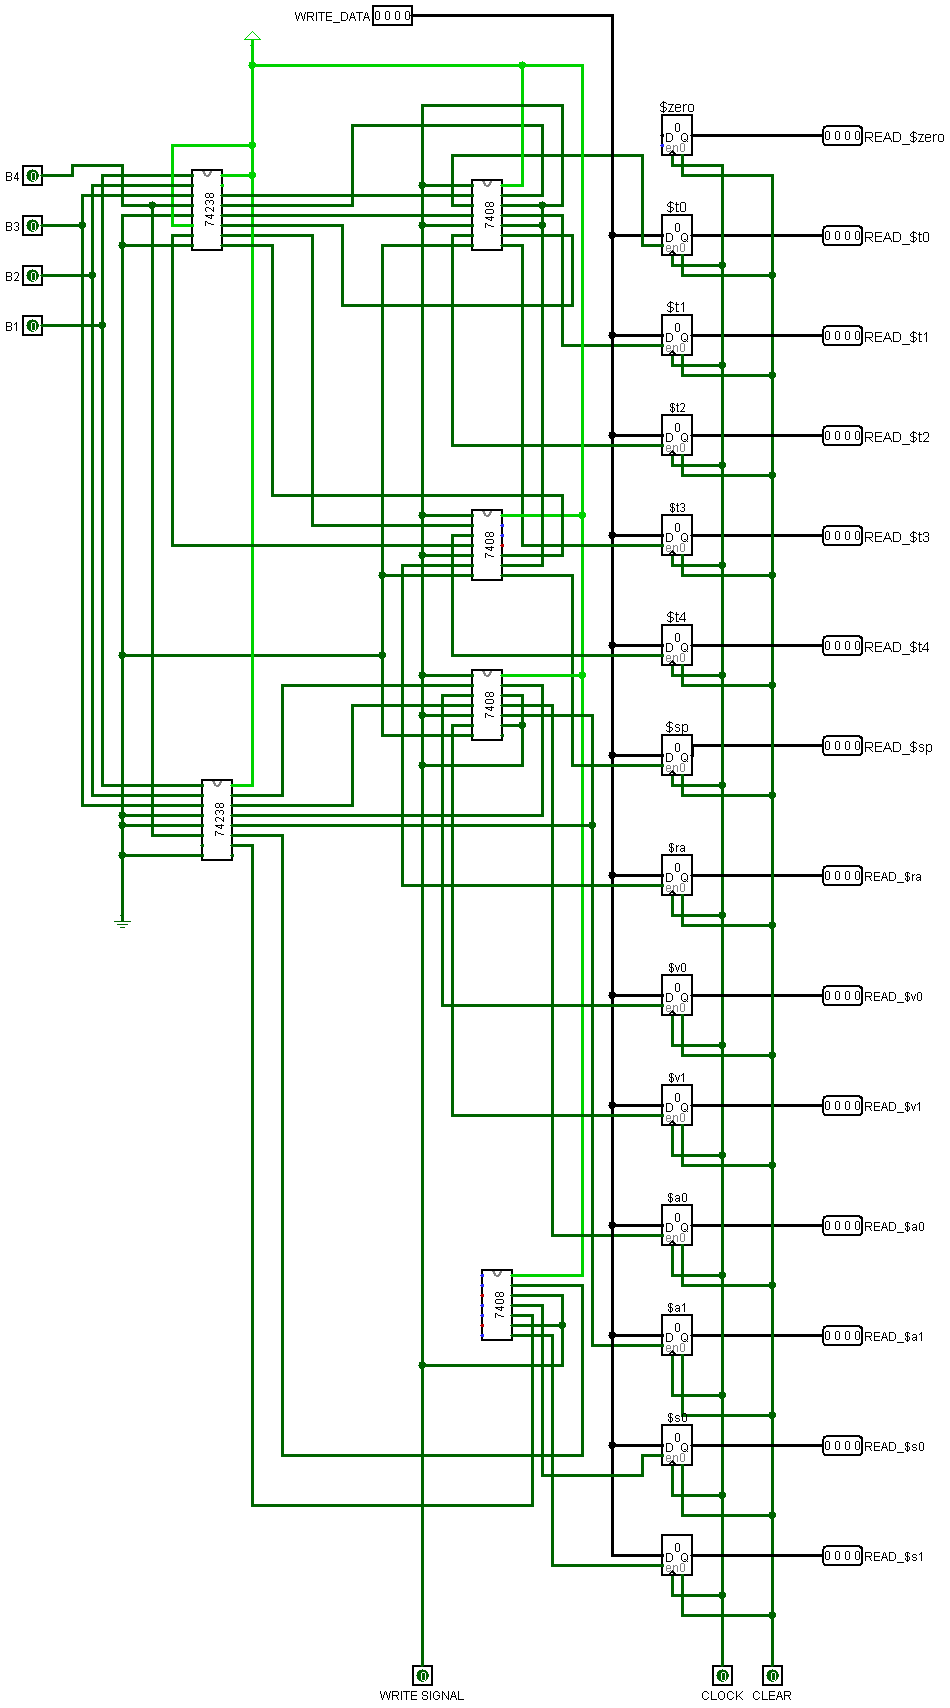
\includegraphics[width = 0.9\textwidth, height = 20cm]{WRITE_REGISTER_CIRCUIT.png}
        \caption{\textbf{Writer}}
        \label{fig:8}
    \end{figure}

    \begin{figure}[H]
        \centering
        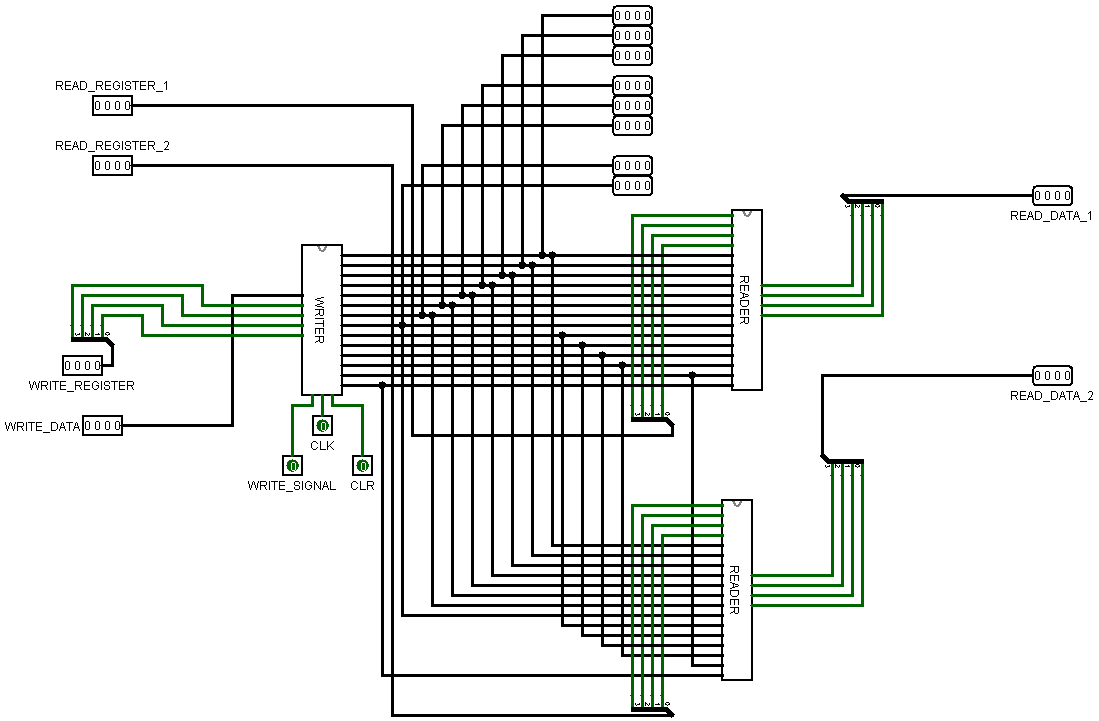
\includegraphics[width = 0.9\textwidth ]{REGISTER_CIRCUIT.png}
        \caption{\textbf{Register Circuit}}
        \label{fig:9}
    \end{figure}
\subsection{ALU}
\subsubsection{ALU Control}
    In this block, the ALUOp is taken out from ALU through a decoder and the output of the decoder is passed to a priority encoder, so that the ALUop is converted to a 3bit MUX Control. The operation we choose from the mux will be output of the ALU.\\

    The ALU implements 7 operations in total. Addition, Subtraction, Logical AND, Logical OR, Logical NOR, Shift Logical Left, Shift Logical Right.

    \begin{tikzpicture}
        \node (dummy) []{};
        \node (mother) [lblock, right of = dummy, xshift = 7cm, below of = dummy, yshift = -7cm]{};
        \node (name) [ right of = mother, xshift = 7cm, ]{\textbf{ALU Control}};
        \node (in1) [io, right of = dummy, xshift = 7cm]{4 bit Opcode};
        \node (dec) [sblock, below of =in1, yshift = -3cm] {4*16 Decoder};
        \node (in2) [io, below of = dec,yshift = -3cm]{OR};
        \node (enc) [sblock, below of =in2, yshift = -3cm] {8*3 Priority Encoder};
        \node (in3) [io, below of =enc, yshift = -3cm]{ALU Control Signal(3 bit ALUOP)};
        \node (mux) [sblock, below of =in3, yshift = -3cm] {8*1 MUX};
        \node (opr) [sblock, right of =mux, xshift = 7cm] {ALU Operation results};
        \node (out1)[io, below of = mux,yshift = -3cm]{Output};
        

        \draw[arrow](in1) -- (dec);
        \draw[arrow](dec) -- (in2);
        \draw[arrow](in2) -- (enc);
        \draw[arrow](enc) -- (in3);
        \draw[arrow](in3) -- (mux);
        \draw[arrow](mux) -- (out1);
        \draw[arrow](name) -- (mother);
        \draw[arrow](opr) -- (mux);
        
    \end{tikzpicture}

    \begin{table}[H]
        \centering
        \begin{tabular}{|c|c|}
            \hline 
            \textbf{Instructions with Opcode} & \textbf{ALUOP} \\
            \hline 
            \textbf{lw(1)}  & \multirow{4}{*}{000} \\
            \cline{1-1} 
            \textbf{add(6)} &  \\
            \cline{1-1} 
            \textbf{sw(9)}   &\\
            \cline{1-1}
            \textbf{addi(B)}  &\\
            
            \hline 
            \hline
            \textbf{sub(0)}   & \multirow{4}{*}{001} \\
            \cline{1-1} 
            \textbf{bneq(2)}  &  \\
            \cline{1-1} 
            \textbf{beq(3)}   &\\
            \cline{1-1}
            \textbf{subi(7)}  &\\
            
            \hline 
            \hline
            \textbf{andi(8)}   & \multirow{2}{*}{010} \\
            \cline{1-1} 
            \textbf{and(F)}  &  \\
             

            \hline 
            \hline
            \textbf{ori(5)}   & \multirow{2}{*}{011} \\
            \cline{1-1} 
            \textbf{or(C)}  &  \\
             
            \hline 
            \hline
            \textbf{nor(A)}   & 100 \\
            
            \hline 
            \hline
            \textbf{srl(D)}   & 101 \\

            \hline 
            \hline
            \textbf{sll(E)}   & 110 \\
            \hline 
              
        \end{tabular}
        \caption{Caption}
        \label{tab:my_label}
    \end{table}

\subsubsection{ALU Operation}

    \begin{figure}[H]
        \centering
        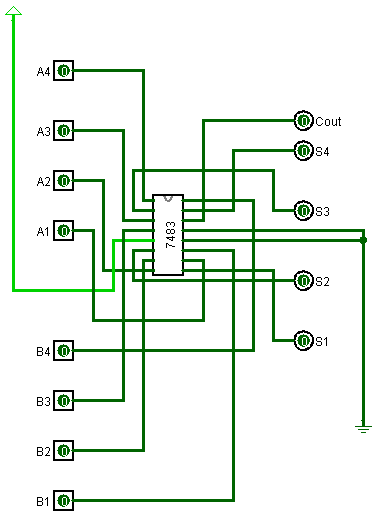
\includegraphics[height = 12cm]{ADDER.png}
        \caption{\textbf{4 bit Adder}}
        \label{fig:10}
    \end{figure}

   

\begin{multicols}{2}

     \begin{figure}[H]
        \centering
        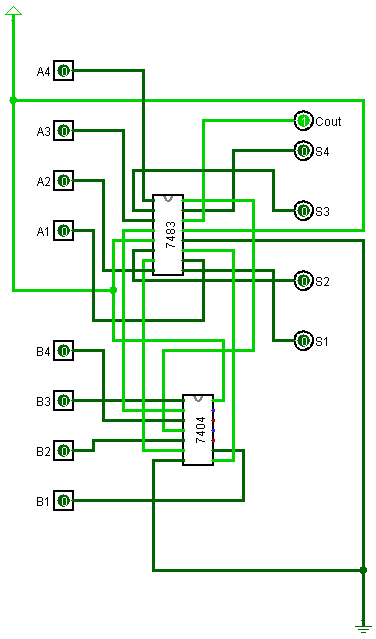
\includegraphics[width = 0.5\textwidth,height = 11cm]{SUBTRACTOR.png}
        \caption{\textbf{4 bit Subtractor}}
        \label{fig:11}
    \end{figure}

    \begin{figure}[H]
        \centering
        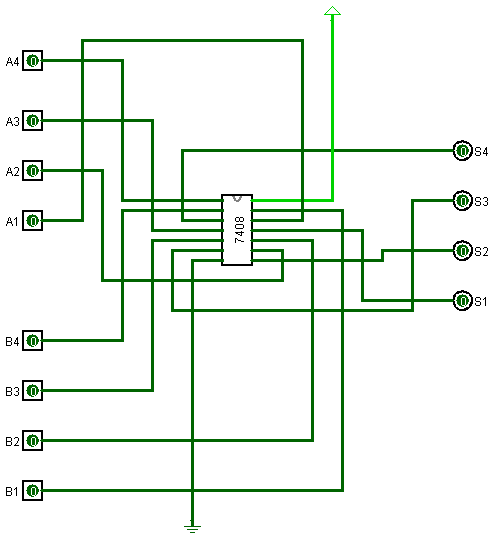
\includegraphics[width = 0.5\textwidth,height = 11cm]{AND.png}
        \caption{\textbf{4 bit AND}}
        \label{fig:12}
    \end{figure}
    
\end{multicols}

\begin{multicols}{2}

     \begin{figure}[H]
        \centering
        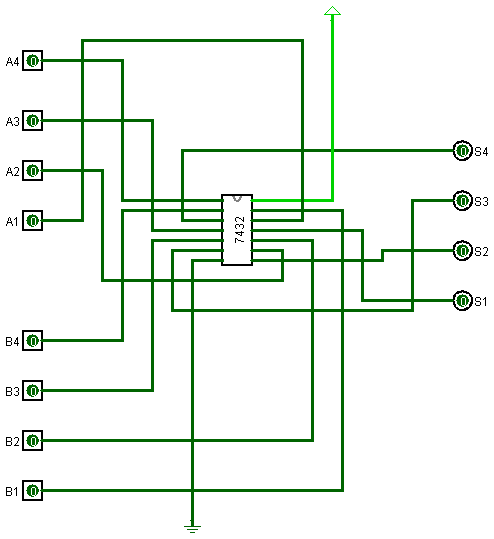
\includegraphics[width = 0.5\textwidth,height = 11cm]{OR.png}
        \caption{\textbf{4 bit OR}}
        \label{fig:13}
    \end{figure}

    \begin{figure}[H]
        \centering
        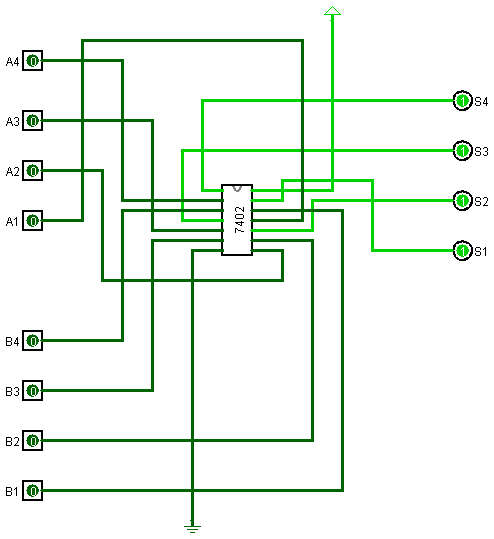
\includegraphics[width = 0.5\textwidth,height = 11cm]{NOR.png}
        \caption{\textbf{4 bit NOR}}
        \label{fig:14}
    \end{figure}
    
\end{multicols}

\begin{multicols}{2}

     \begin{figure}[H]
        \centering
        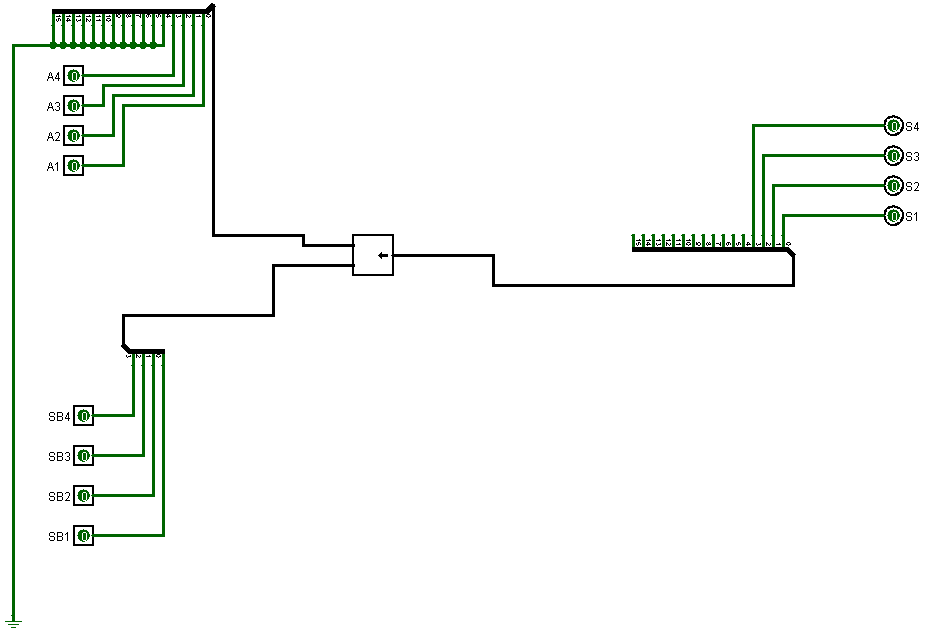
\includegraphics[width = 0.5\textwidth,height = 11cm]{SLL.png}
        \caption{\textbf{4 bit left Shifter}}
        \label{fig:15}
    \end{figure}

    \begin{figure}[H]
        \centering
        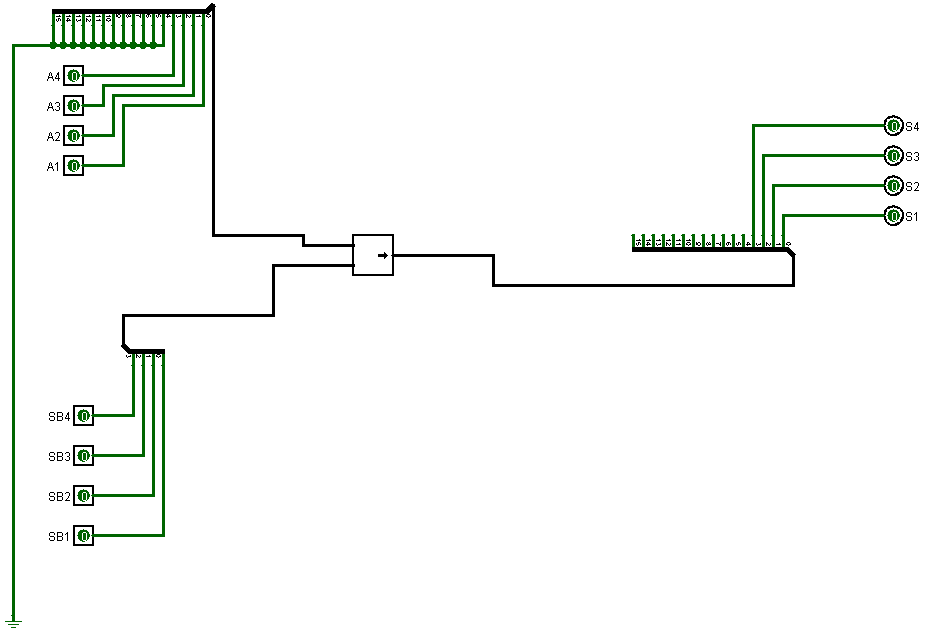
\includegraphics[width = 0.5\textwidth,height = 11cm]{SRL.png}
        \caption{\textbf{4 bit right Shifter}}
        \label{fig:16}
    \end{figure}
    
\end{multicols}

    
    \begin{figure}[H]
        \centering
        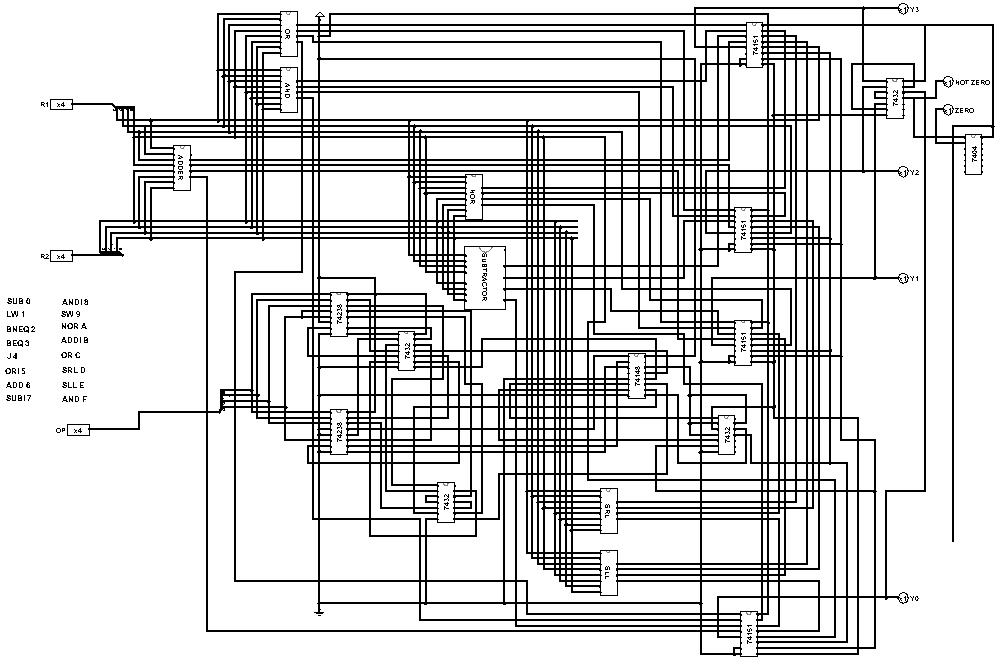
\includegraphics[width = 0.9\textwidth,height = 11cm]{ALU.png}
        \caption{\textbf{4 bit ALU}}
        \label{fig:17}
    \end{figure}

    \begin{figure}[H]
        \centering
        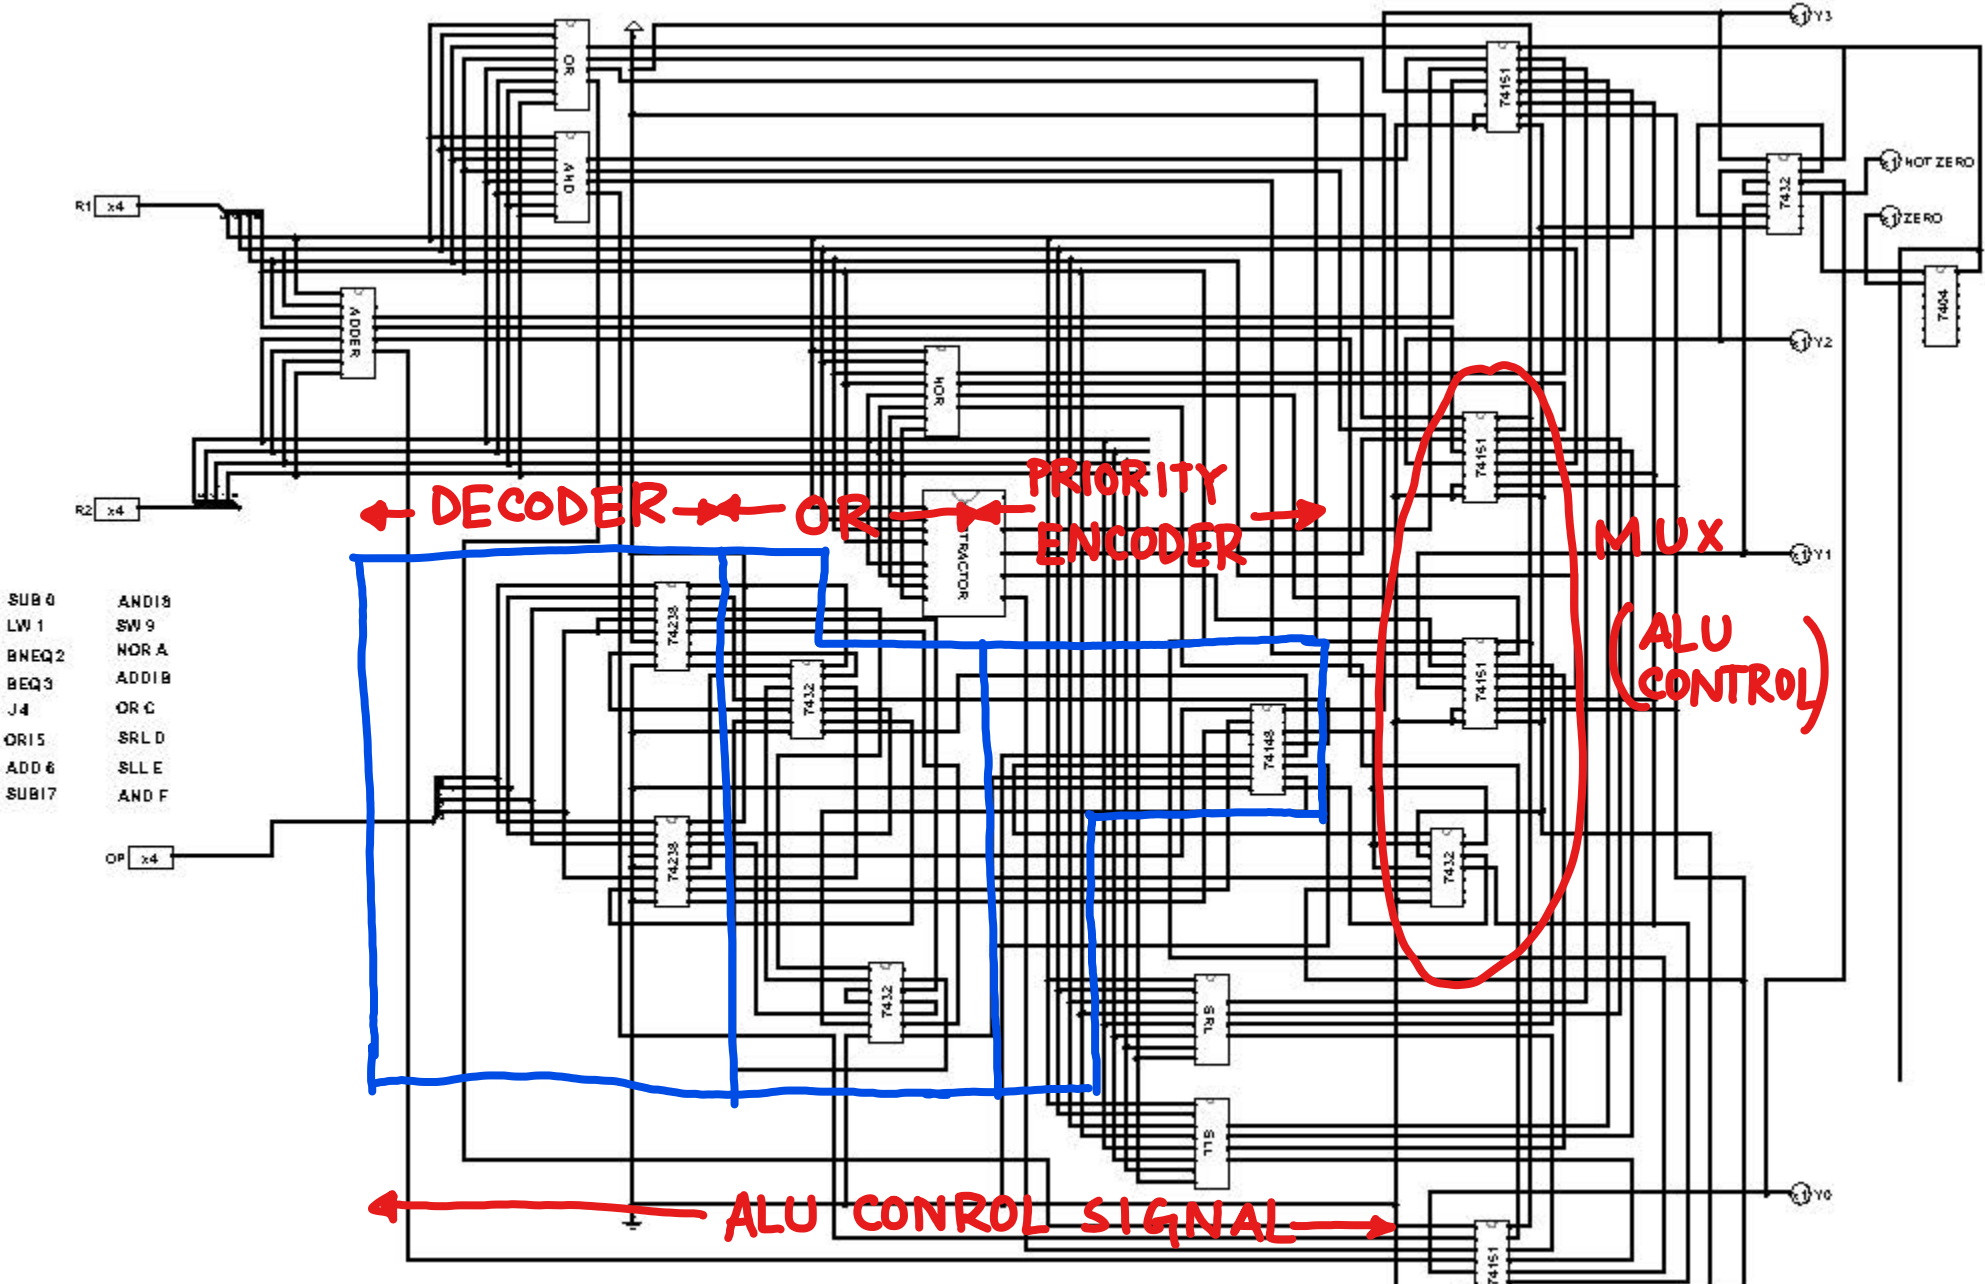
\includegraphics[width = 0.9\textwidth]{ALUMARK.png}
        \caption{\textbf{ALU Control Marked}}
        \label{fig:18}
    \end{figure}

    
\subsection{Data Memory}
    In the Data memory, we have a \textit{RAM} that takes a \textbf{4 bit address} as input and \textbf{4 bit data} as output. Here the 
    \textbf{4 bit address} is the \textbf{Memory address} in which we want to store our data, either by \textit{store word} or by \textit{stack}, while each \textbf{4 bit data } denotes the \textbf{data kept in the input address}.\\
    \begin{itemize}
        \item Whether to read an \textbf{address data} from the data memory to load on register is activated by control \textbf{MemRead}
        \item Whether to transfer an \textbf{address data} from the data memory to load on register is activated by control \textbf{MemtoReg}
        \item Whether to write a \textbf{data} to a certain \textbf{address} of the data memory to store is activated by control \textbf{MemWrite}\\
    \end{itemize}

    \begin{figure}[H]
        \centering
        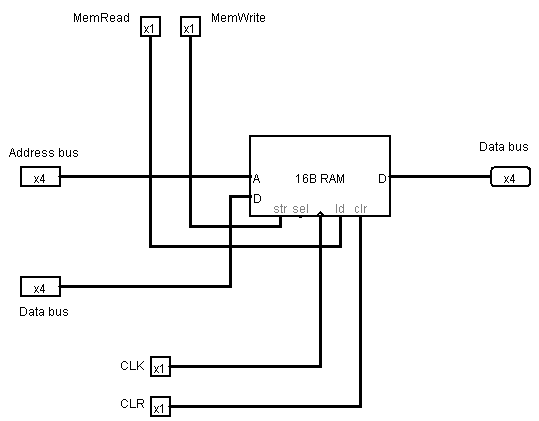
\includegraphics[width = 0.9\textwidth]{DATA MEMORY.png}
        \caption{\textbf{Data Memory}}
        \label{fig:19}
    \end{figure}
\subsection{Branching and Program Counter}

    For a general instruction, the program counter should increase by 1 after execution, unless we are up for a jump.\\
    Branching(beq,bneq) are called conditional jumps and general Jumps (j,jal,jr) are unconditional.\\
    In case of branching or Jumping, the program counter shall proceed to a label that has been called for jump. Else the program counter will be incremented by 1 for each instruction.\\ \\
    

\section{How to write and execute a program in this machine}
    \textbf{Step 1: } At first we have to run the user programmed MIPS code (which is to be preserved in a text file input.txt) and then parsed through the assembler. This will generate a hex code of a set of mips instruction in some file output.txt) \\ \\
    \textbf{Step 2: } In case of software simulation the output.txt code will be loaded to the instruction memory( \textit{EEPROM} ) while in case of hardware implementation, the output hex file has to be passed as a group of hex strings to the \textit{ATMEGA32} for instruction memory. The \textit{EEPROM} of \textit{ATMEGA32} is implemented in this case\\ \\
    \textbf{Step 3: } At each instruction the clock pulse has to be provided in both cases. Each clock pulse will either forward the registers to next instruction or branch it back or jump to another instruction based on the instruction provided to it.\\ \\
    \textbf{Step 4: } All the register values can be shown in software simulation after an instruction is executed, but only output register can shown in hardware implementation.
    The Program counter can be shown in both instructions.\\ \\ 
    
\section{Special Features Implemented}

\subsection{User programmable Push Pop in stack : }

We have added the stack pointer in our software (\textbf{\$sp}). It will rise from the bottom of Data Memory whenever user will push a data, and remove data from top whenever popped. The command has to be given in the following format.

\begin{verbatim}

    addi $sp,$sp,-1 #allocating a space for stack pointer for pushing the data
    sw $t0,0($sp) #pushing one data (data in $t0)in our stack pointer
    lw $t1,0($sp) #popping the data from our stack pointer and assign it to $t2
    addi $sp,$sp,1 #deallocating the allocated segment
    
\end{verbatim}

\subsection{User programmable function writing : }

We have also implemented the procedure calling in our software implementation. Instructions \textbf{jal}(Jump and Link) and jr(Jump return) has been implemented.\\
Any jal command within 16 instructions work.\\
Additionally, for the purpose to serve the procedure calling additional registers are implemented. Those are \textbf{\$ra,\$ao,\$a1,\$v0,\$v1,\$s0,\$s1}. The command has to be given in the following format.\\

\textbf{C code: }
\begin{verbatim}

    int leaf(int a, int b){

        return a+b;
    }

    int main{

        int x=5,y=6;
        int z = leaf(x,y);
        
    }
    
    
\end{verbatim}

\textbf{Eqivalent MIPS code: }
\begin{verbatim}
    addi $a0,$zero,5
    addi $a1,$zero,6
    jal leaf
    add $t0,$s0,$zero

    leaf:
    add $v0,$a0,$a1
    add $s0,$v0,$zero
    jr $ra
\end{verbatim}
\section{Function of Different Control Signals} 

\subsection{RegDst : }

RegDst controls a mux to select from either BIT3-BIT0 or BIT7-BIT4 to feed to Writing Register of the Instruction Memory.
\subsection{Branch Equal : }

Branch Equal undergoes an AND operation with ALU Zero Flag to assertain whether the Branching is satisfied on Equal values or not. Based on the results it may execute a conditional Jump.
\subsection{Branch not Equal : }

Branch Equal undergoes an AND operation with ALU NotZero Flag to assertain whether the Branching is satisfied on inequal values or not. Based on the results it may execute a conditional Jump.
\subsection{Jump : }

Jumping on a label is unconditional. Jump activates the program counter to proceed to a label unconditionally.
\subsection{MemRead : }

While loading a data to register from a certain addres in Data Memory, memory has to be read. MemRead activates the Data Memory to enable data reading
\subsection{MemWrite : }

While storing a data from a register to a certain address in data memory, memory has to be written. MemWrite enables the data memory for writing data to a specified address.
\subsection{MemtoReg : }

Only reading memory is not enough to write a value obtained from memory to register, for which, MemToReg will activate a mux to whether write the value to the register or not.
\subsection{ALUSrc : }

ALUSrc activates a mux that will select either of register data or immediate data to be passed to ALU. I-type instruction have an ALUSrc 1, to select immediate value for writing data. Or it may be 0, which will redirect it to select the value passing from the Register. 
\subsection{RegWrite : }

RegWrite enables the write signal for the register. RegWrite from Control unit or RegWrite from jal activates the write signal. If jal activates write signal, data will be written specifically to \$ra. 
\subsection{JR : }
JR activates a mux to chose whether the jump is a branch jump, or unconditional jump or the return jump. Branch Jump passes through the first mux, Unconditional Jump passes throgh the second mux with the output of Branch Mux. While the output goes to another mux with the jump return.

\section{IC's with their Count: }

\subsection{Software}

\begin{itemize}
    \item \textbf{IC 7402: Quad 2input NOR : } 1
    \item \textbf{IC 7404: Hex 1input NOT : } 4
    \item \textbf{IC 7408: Quad 2input OR : } 8
    \item \textbf{IC 7432: Quad 2input AND : } 12
    \item \textbf{IC 7483: 4 bit adder : } 4
    \item \textbf{IC 74148: 8*3 Priority Encoder : } 1
    \item \textbf{IC 74151: 8*1 MUX : } 20
    \item \textbf{IC 74157: Quad 2*1 MUX : } 20
    \item \textbf{IC 74238: 3*8 Decoder : } 6
    \item \textbf{IC 74273: Register : } 16
    \item \textbf{EEPROM : } 1
    \item \textbf{RAM : } 1
    \item \textbf{Left Shifter : } 1
    \item \textbf{Right Shifter : } 1
    \item \textbf{Clock : } 1
    
\end{itemize}

\subsection{Hardware}

\begin{itemize}
    %\item \textbf{IC 7402: Quad 2input NOR : } 1
    \item \textbf{IC 7404: Hex 1input NOT : } 1
    \item \textbf{IC 7408: Quad 2input OR : } 1
    \item \textbf{IC 7432: Quad 2input AND : } 2
    %\item \textbf{IC 7483: 4 bit adder : } 4
    %\item \textbf{IC 74148: 3*8 Priority Encoder : } 1
    %\item \textbf{IC 74151: 8*1 MUX : } 20
    %\item \textbf{IC 74157: Quad 2*1 MUX : } 20
    %\item \textbf{IC 74238: 8*3 Decoder : } 6
    \item \textbf{IC 74273: Register : } 1
    %\item \textbf{EEPROM : } 1
    %\item \textbf{RAM : } 1
    \item \textbf{Push Switch : } 1
    \item \textbf{ATMEGA32 : } 5
    \item \textbf{Clock : } 1
    
\end{itemize}

\section{Discussion}
In case of hardware implementation, all the equipments were tested individually and then we tried to combine them. Unfortunately the D flip flop was not being able to generate proper PC even though we used falling edge configuration to avoid debouncing. One possible reason is the given clock was not being able to sync with the clocks of Atmega32. Due to this reason, register values were not stored and only immediate or R/I type instructions were performed successfully.

All the wires and ICs were attached carefully. Wires were given connection after thorough cross checking. Still there remained some errors and our project was not fully successful.

\section{References}
\begin{enumerate}
    \item \textbf{All images in full resolution : }  \href{https://drive.google.com/drive/folders/1C4mjVRfIBffSrGZZEEEl85NEq3H7LgYy?usp=share_link}{\textcolor{blue}{\underline{IMAGES}}}
    \item \textbf{Assembler code: }
    \href{https://drive.google.com/file/d/1huQxe8--XFIrjrw-dRG1LzcaEkW_kyHk/view?usp=share_link}{\textcolor{blue}{\underline{ASSEMBLER}}}
     
\end{enumerate}


\end{document}

